\documentclass{standalone}
\usepackage{tikz}
\usetikzlibrary{patterns, positioning}
\usepackage[sfdefault]{ClearSans} %% option 'sfdefault' activates Clear Sans as the default text font
\usepackage[T1]{fontenc}

\begin{document}
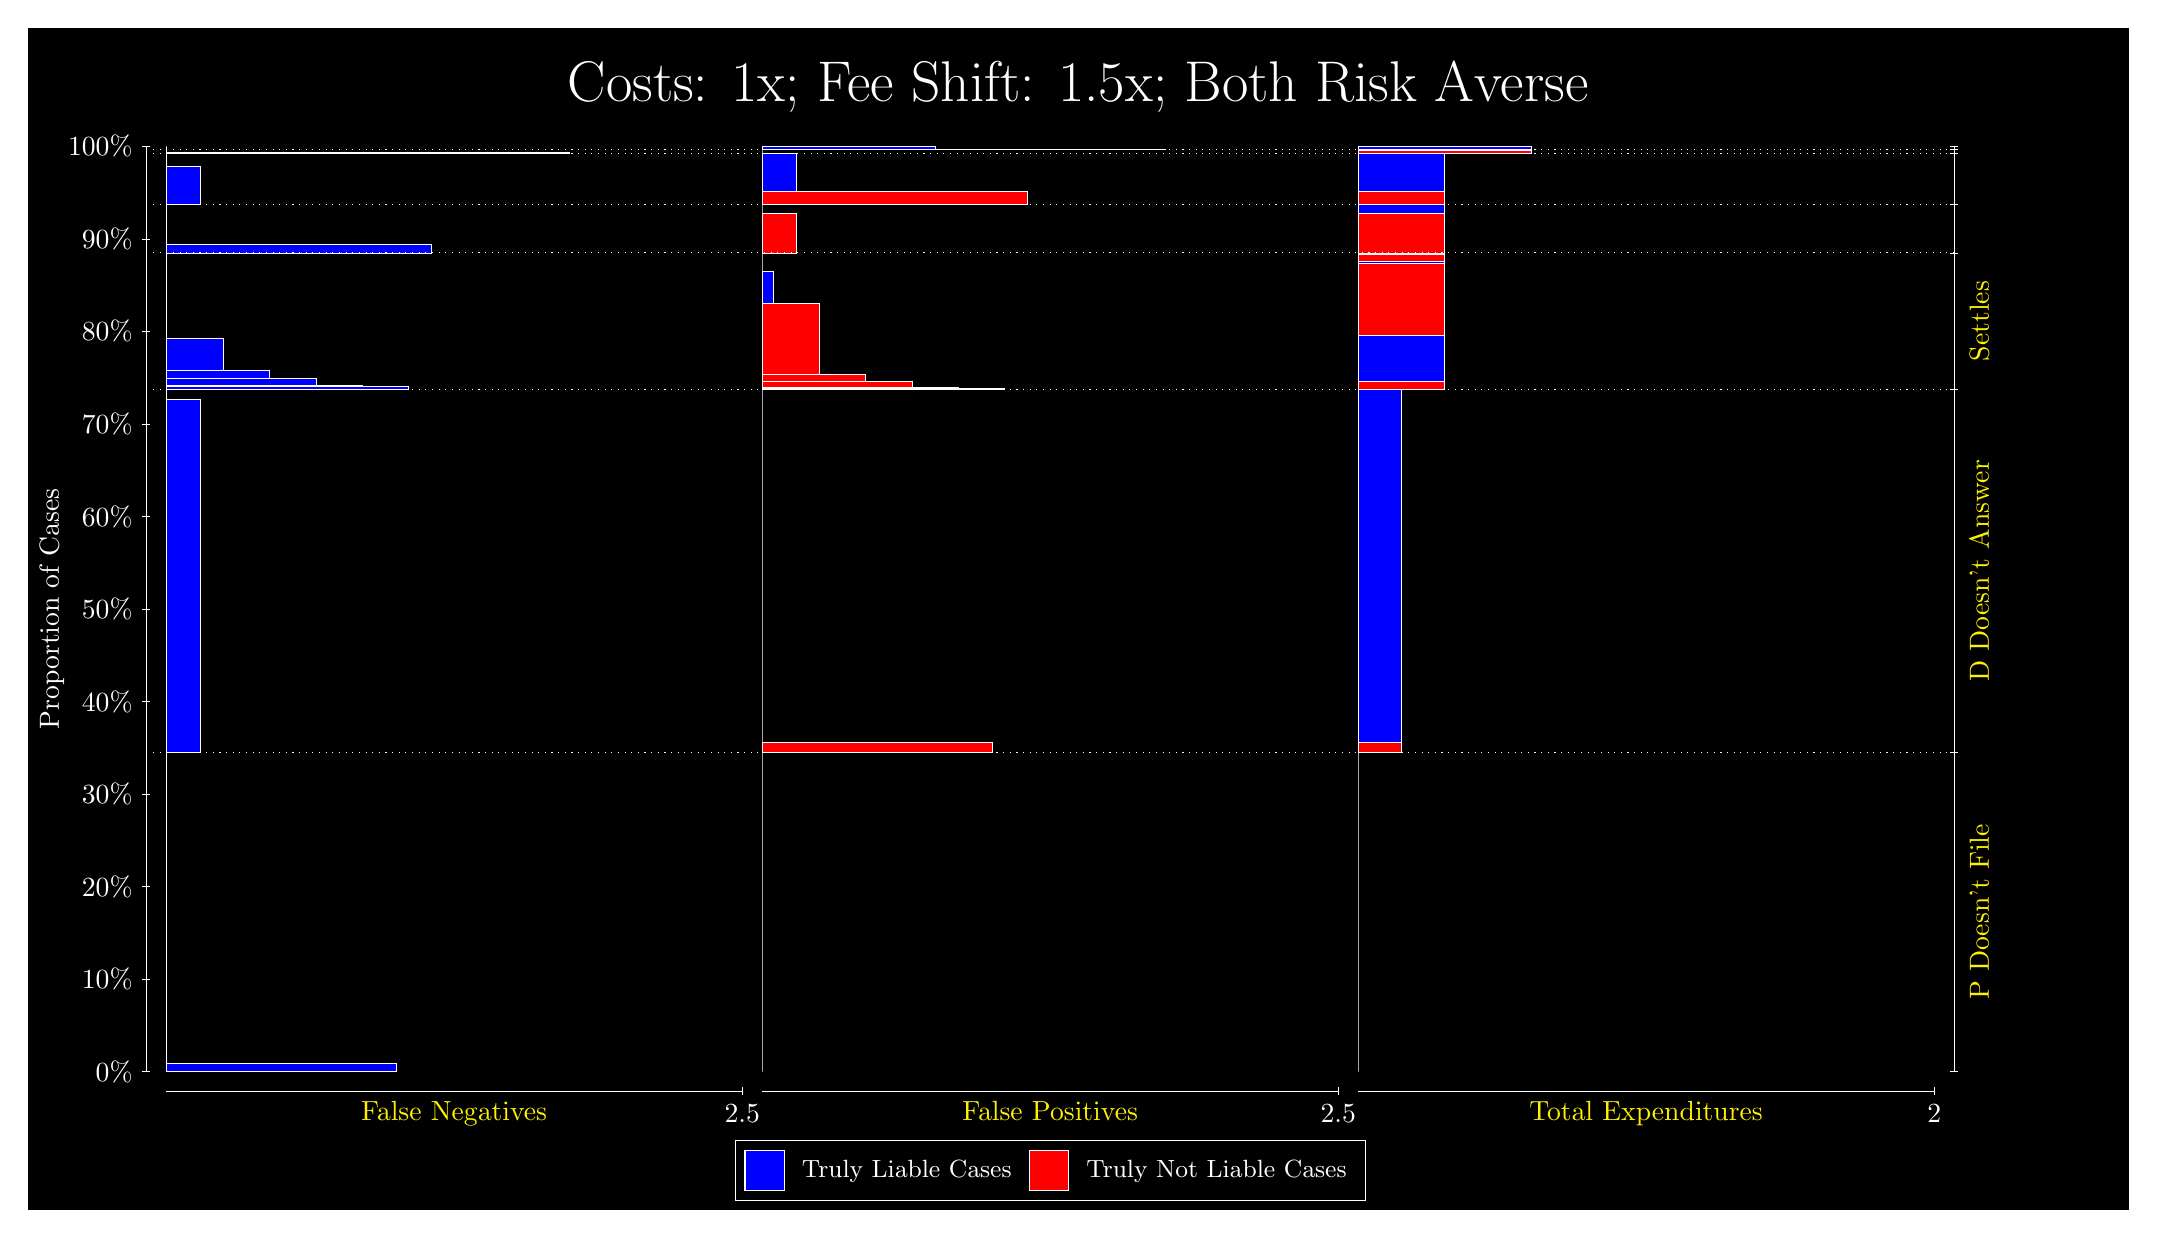
\begin{tikzpicture}
\draw[fill=black] (0,0) rectangle (26.667,15);
\draw[text=white] (0,13.5) rectangle (26.667,15) node[midway] {\huge Costs: 1x; Fee Shift: 1.5x; Both Risk Averse};
\draw[white, very thin] (1.5,1.75) -- (1.5,13.5);
\node[rotate=90, text=white, anchor=center] at (0.3, 7.625) {Proportion of Cases};
\draw[white, very thin] (1.45,1.75) -- (1.55,1.75);
\node[text=white, anchor=east] at (1.45, 1.75) {0\%};
\draw[white, very thin] (1.45,2.925) -- (1.55,2.925);
\node[text=white, anchor=east] at (1.45, 2.925) {10\%};
\draw[white, very thin] (1.45,4.1) -- (1.55,4.1);
\node[text=white, anchor=east] at (1.45, 4.1) {20\%};
\draw[white, very thin] (1.45,5.275) -- (1.55,5.275);
\node[text=white, anchor=east] at (1.45, 5.275) {30\%};
\draw[white, very thin] (1.45,6.45) -- (1.55,6.45);
\node[text=white, anchor=east] at (1.45, 6.45) {40\%};
\draw[white, very thin] (1.45,7.625) -- (1.55,7.625);
\node[text=white, anchor=east] at (1.45, 7.625) {50\%};
\draw[white, very thin] (1.45,8.8) -- (1.55,8.8);
\node[text=white, anchor=east] at (1.45, 8.8) {60\%};
\draw[white, very thin] (1.45,9.975) -- (1.55,9.975);
\node[text=white, anchor=east] at (1.45, 9.975) {70\%};
\draw[white, very thin] (1.45,11.15) -- (1.55,11.15);
\node[text=white, anchor=east] at (1.45, 11.15) {80\%};
\draw[white, very thin] (1.45,12.325) -- (1.55,12.325);
\node[text=white, anchor=east] at (1.45, 12.325) {90\%};
\draw[white, very thin] (1.45,13.5) -- (1.55,13.5);
\node[text=white, anchor=east] at (1.45, 13.5) {100\%};

\draw[white, very thin] (24.457,1.75) -- (24.457,13.5);
\draw[white, very thin] (24.407,1.75) -- (24.507,1.75);
\node[anchor=west] at (24.407, 1.75) {};
\draw[white, very thin] (24.407,5.8014) -- (24.507,5.8014);
\node[anchor=west] at (24.407, 5.8014) {};
\draw[white, very thin] (24.407,10.416) -- (24.507,10.416);
\node[anchor=west] at (24.407, 10.416) {};
\draw[white, very thin] (24.407,12.148) -- (24.507,12.148);
\node[anchor=west] at (24.407, 12.148) {};
\draw[white, very thin] (24.407,12.76) -- (24.507,12.76);
\node[anchor=west] at (24.407, 12.76) {};
\draw[white, very thin] (24.407,13.413) -- (24.507,13.413);
\node[anchor=west] at (24.407, 13.413) {};
\draw[white, very thin] (24.407,13.46) -- (24.507,13.46);
\node[anchor=west] at (24.407, 13.46) {};
\draw[white, very thin] (24.407,13.5) -- (24.507,13.5);
\node[anchor=west] at (24.407, 13.5) {};

\draw[white, very thin, fill=blue] (1.75,1.75) rectangle (4.6775,1.858);
\draw[white, very thin, fill=red] (1.75,1.858) rectangle (1.75,5.8014);
\draw[white, very thin, fill=blue] (1.75,5.8014) rectangle (2.1891,10.292);
\draw[white, very thin, fill=red] (1.75,10.292) rectangle (1.75,10.416);
\draw[white, very thin, fill=blue] (1.75,10.416) rectangle (4.8239,10.45);
\draw[white, very thin, fill=blue] (1.75,10.45) rectangle (4.2384,10.47);
\draw[white, very thin, fill=blue] (1.75,10.47) rectangle (3.6529,10.551);
\draw[white, very thin, fill=blue] (1.75,10.551) rectangle (3.0674,10.655);
\draw[white, very thin, fill=blue] (1.75,10.655) rectangle (2.4819,11.056);
\draw[white, very thin, fill=red] (1.75,11.056) rectangle (1.75,12.148);
\draw[white, very thin, fill=blue] (1.75,12.148) rectangle (5.1167,12.257);
\draw[white, very thin, fill=red] (1.75,12.257) rectangle (1.75,12.76);
\draw[white, very thin, fill=blue] (1.75,12.76) rectangle (2.1891,13.248);
\draw[white, very thin, fill=red] (1.75,13.248) rectangle (1.75,13.413);
\draw[white, very thin, fill=blue] (1.75,13.413) rectangle (6.8732,13.42);
\draw[white, very thin, fill=red] (1.75,13.42) rectangle (1.75,13.46);
\draw[white, very thin, fill=red] (1.75,13.46) rectangle (1.75,13.467);
\draw[white, very thin, fill=blue] (1.75,13.467) rectangle (1.75,13.5);
\draw[white, very thin, fill=red] (9.3189,1.75) rectangle (9.3189,5.6934);
\draw[white, very thin, fill=blue] (9.3189,5.6934) rectangle (9.3189,5.8014);
\draw[white, very thin, fill=red] (9.3189,5.8014) rectangle (12.246,5.9258);
\draw[white, very thin, fill=blue] (9.3189,5.9258) rectangle (9.3189,10.416);
\draw[white, very thin, fill=red] (9.3189,10.416) rectangle (12.393,10.422);
\draw[white, very thin, fill=red] (9.3189,10.422) rectangle (11.807,10.442);
\draw[white, very thin, fill=red] (9.3189,10.442) rectangle (11.222,10.517);
\draw[white, very thin, fill=red] (9.3189,10.517) rectangle (10.636,10.603);
\draw[white, very thin, fill=red] (9.3189,10.603) rectangle (10.051,11.507);
\draw[white, very thin, fill=blue] (9.3189,11.507) rectangle (9.4652,11.908);
\draw[white, very thin, fill=blue] (9.3189,11.908) rectangle (9.3189,12.148);
\draw[white, very thin, fill=red] (9.3189,12.148) rectangle (9.758,12.651);
\draw[white, very thin, fill=blue] (9.3189,12.651) rectangle (9.3189,12.76);
\draw[white, very thin, fill=red] (9.3189,12.76) rectangle (12.686,12.925);
\draw[white, very thin, fill=blue] (9.3189,12.925) rectangle (9.758,13.413);
\draw[white, very thin, fill=red] (9.3189,13.413) rectangle (9.3189,13.454);
\draw[white, very thin, fill=blue] (9.3189,13.454) rectangle (9.3189,13.46);
\draw[white, very thin, fill=red] (9.3189,13.46) rectangle (14.442,13.467);
\draw[white, very thin, fill=blue] (9.3189,13.467) rectangle (11.515,13.5);
\draw[white, very thin, fill=red] (16.888,1.75) rectangle (16.888,5.6934);
\draw[white, very thin, fill=blue] (16.888,5.6934) rectangle (16.888,5.8014);
\draw[white, very thin, fill=red] (16.888,5.8014) rectangle (17.437,5.9258);
\draw[white, very thin, fill=blue] (16.888,5.9258) rectangle (17.437,10.416);
\draw[white, very thin, fill=red] (16.888,10.416) rectangle (17.986,10.517);
\draw[white, very thin, fill=blue] (16.888,10.517) rectangle (17.986,11.104);
\draw[white, very thin, fill=red] (16.888,11.104) rectangle (17.986,12.009);
\draw[white, very thin, fill=blue] (16.888,12.009) rectangle (17.986,12.042);
\draw[white, very thin, fill=red] (16.888,12.042) rectangle (17.986,12.128);
\draw[white, very thin, fill=blue] (16.888,12.128) rectangle (17.986,12.148);
\draw[white, very thin, fill=red] (16.888,12.148) rectangle (17.986,12.651);
\draw[white, very thin, fill=blue] (16.888,12.651) rectangle (17.986,12.76);
\draw[white, very thin, fill=red] (16.888,12.76) rectangle (17.986,12.925);
\draw[white, very thin, fill=blue] (16.888,12.925) rectangle (17.986,13.413);
\draw[white, very thin, fill=red] (16.888,13.413) rectangle (19.083,13.454);
\draw[white, very thin, fill=blue] (16.888,13.454) rectangle (19.083,13.46);
\draw[white, very thin, fill=red] (16.888,13.46) rectangle (19.083,13.467);
\draw[white, very thin, fill=blue] (16.888,13.467) rectangle (19.083,13.5);
\draw[white, dotted] (1.5,5.8014) -- (24.457,5.8014);
\draw[white, dotted] (1.5,10.416) -- (24.457,10.416);
\draw[white, dotted] (1.5,12.148) -- (24.457,12.148);
\draw[white, dotted] (1.5,12.76) -- (24.457,12.76);
\draw[white, dotted] (1.5,13.413) -- (24.457,13.413);
\draw[white, dotted] (1.5,13.46) -- (24.457,13.46);
\draw[white, very thin] (1.75,1.5) -- (9.0689,1.5);
\node[text=yellow, anchor=north] at (5.4094, 1.5) {False Negatives};
\draw[white, very thin] (9.0689,1.45) -- (9.0689,1.55);
\node[text=white, anchor=north] at (9.0689, 1.45) {2.5};

\draw[white, very thin] (9.3189,1.5) -- (16.638,1.5);
\node[text=yellow, anchor=north] at (12.978, 1.5) {False Positives};
\draw[white, very thin] (16.638,1.45) -- (16.638,1.55);
\node[text=white, anchor=north] at (16.638, 1.45) {2.5};

\draw[white, very thin] (16.888,1.5) -- (24.207,1.5);
\node[text=yellow, anchor=north] at (20.547, 1.5) {Total Expenditures};
\draw[white, very thin] (24.207,1.45) -- (24.207,1.55);
\node[text=white, anchor=north] at (24.207, 1.45) {2};

\node[text=yellow, centered, rotate=90] at (24.777, 3.7757) {P Doesn't File};
\node[text=yellow, centered, rotate=90] at (24.777, 8.1087) {D Doesn't Answer};
\node[text=yellow, centered, rotate=90] at (24.777, 11.282) {Settles};





\draw (12.978300999999998,1.5) node[draw=none] (baseCoordinate) {};
\begin{scope}[align=center]
        \matrix[scale=0.5, draw=white, below=0.5cm of baseCoordinate, nodes={draw}, column sep=0.1cm]{
            \node[rectangle, draw, minimum width=0.5cm, minimum height=0.5cm, fill=blue] {}; &
            \node[draw=none, font=\small, text=white] (B) {Truly Liable Cases}; &
            \node[rectangle, draw, minimum width=0.5cm, minimum height=0.5cm, fill=red] {}; &
            \node[draw=none, font=\small, text=white] (B) {Truly Not Liable Cases}; \\
            };
\end{scope}

\end{tikzpicture}
\end{document}